\section{Roaming definition}

\-\hspace{0.5cm} Roaming consists in making calls via your cell phone or smartphone, sending, and receiving messages (\acs{SMS}, \acs{MMS}), and connecting to the Internet (browsing, social networks, emails, etc.), but via a different operator than the one to which you subscribe. The roaming is used abroad, we speak of international roaming. For this purpose, Orange France have signed bi-lateral agreements with their international counterparts, so that their users can use their cell phone as well as their tablet and \acs{PC}, regardless of the country they are in (\acs{GSM}, \acs{GPRS}, \acs{3G}, \acs{4G} \acs{LTE}, \acs{VOLTE} and \acs{5G} \acs{NSA}). 

\begin{itemize}
    \setlength\itemsep{0.2em}
    \item Roaming IN (Inbound): Customers of foreign operators can traffic under Orange France network.  
    \item Roaming OUT (Outbound): Orange France customers can traffic on the networks of foreign operators. (See annex 3 \cite{annexes}) 
\end{itemize}

During roaming, many files and information about billing, fraud are being exchanged between the roaming partners. (See annex 4 \cite{annexes})  \\

\section{Roaming Sponsor}
\-\hspace{0.5cm} As developing international roaming coverage could take years, The Roaming Sponsor offer allows Operators (\acs{MNO} or Full \acs{MVNO}) with their own core network to benefit from Orange's international roaming coverage (more than 200 destinations). Offer the Orange quality of service to the operators’ subscribers. Roaming Sponsor is based on a multi-\acs{IMSI} solution and is transparent for the subscribers who keep their phone number. \\

In Roaming situation, Sponsored Network Subscribers are using dedicated Orange France \acs{IMSI} range (ex: 208 0115)\\

Routing of Signaling and Data flows from \acs{VPLMN} through the Sponsor Network \cite{roaming-sponsor} (See Annex 5 \cite{annexes})\\

\begin{figure}[H]
    \centering
    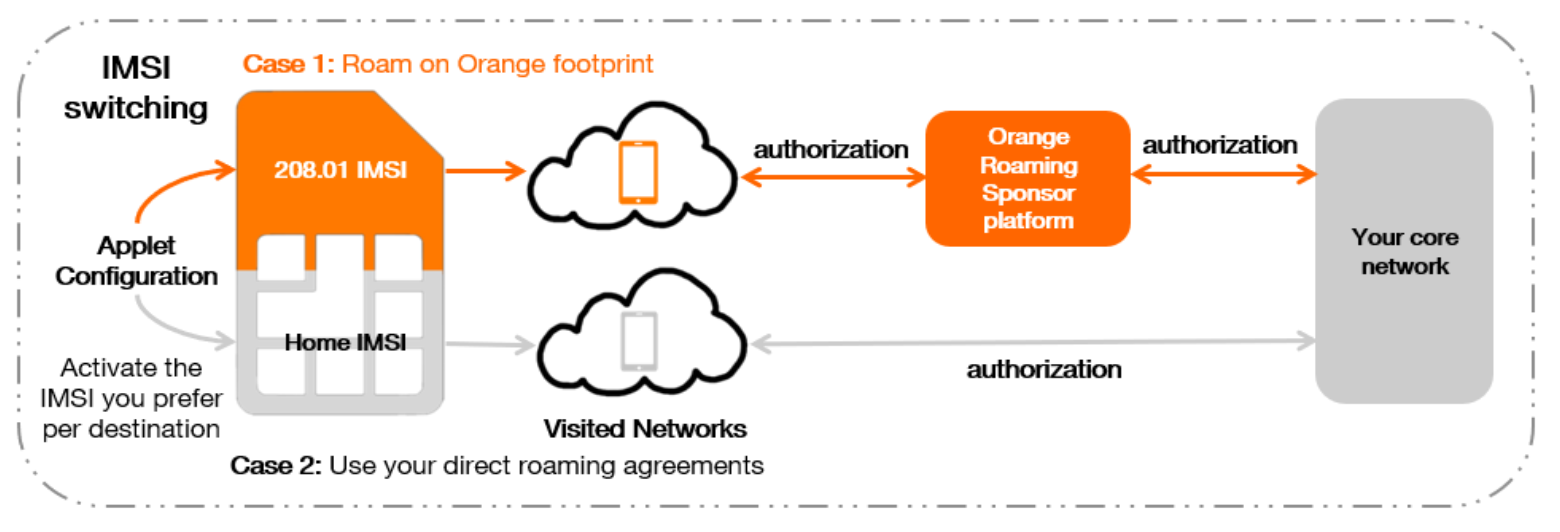
\includegraphics[scale=0.35]{part2/romi.png}
\caption{Roaming Sponsor IMSI Change Process}
\end{figure}

\section{Roaming Hub}
\-\hspace{0.5cm} A roaming hub is a one-stop-shop service that offers client operators accelerated global roaming through simplified implementation and reduced operating costs. The hub enables roaming among all clients of the hub and is an alternative to the current model of effort-intensive bilateral roaming agreements and implementations. The roaming hub provides the clients operator with (see annex 6 \cite{annexes}):
\begin{itemize} 
    \setlength\itemsep{0.2em}
    \item A single agreement with the hub.
    \item A single connection point to the hub.
    \item Provisioning, testing, and troubleshooting support.
    \item Consolidated/Cascade billing (currently being evaluated for future requirement).
    \item Prepaid signaling support.
    \item Fraud prevention and mitigation mechanisms. 
\end{itemize}

An established roaming hub provides mobile operators access to many of the world’s largest roaming networks and can pursue specific non-member networks on behalf of its member operators. New members enjoy rapid expansion of a roaming footprint, while existing members benefit from lower aggregate costs to expand roaming access to new markets and regions with smaller operators.\\

As Roaming bilateral services opening is complicated, costly and take time to reach the market, Orange France has decided to deploy a roaming hub to facilitate roaming opening for Orange affiliates and wholesale market. \cite{roaming-hub} \\

\section{SIGOS remote testing}
\-\hspace{0.5cm} SIGOS is a leading company with over 500 network operators in 156 countries, including the top 100 mobile networks. The company has developed an impressive suite of technology and products that deliver great value to global telecom operators.\\

\acs{SIM} multiplexing is a technology by SIGOS that can handle thousands of \acs{SIM} and \acs{USIM} cards in cascade-style \acs{SIM} card boards. The subscriber information of a \acs{SIM} card is read out by the system and transmitted via a \acs{LAN}/\acs{WAN} network to any test location required. Each card may be virtually transmitted to any location without even a single card having to be moved physically.\\

For outbound roaming testing SIGOS offers the Global Roaming Test Service. \acs{GRTS} allows mobile network operators to activate their own \acs{SIM} cards via the Internet in mobile test stations in remote countries and verify that all services are available for their roaming customers. \cite{sigos} \\ 

\section{\acs{GSM} Association}   

\-\hspace{0.5cm} Founded in 1987, the \acs{GSM} Association brings together nearly 750 licensed mobile operators all around the world, along with approximately 200 manufacturers and suppliers.\\

This association plays a pivotal role in the development of the \acs{GSM} platform and associated services worldwide, by providing a framework for exchanges between operators (standard contracts, summary of operator information in a standardized format, etc.). The primary role of \acs{GSMA} is to ensure global and simple accessibility to mobile services users and to offer an infocenter gathering information from affiliated operators (contacts, services, rates, etc.) \cite{gsma} \\

\section{MACH, Data Clearing House}

\-\hspace{0.5cm} Each mobile operator worldwide is affiliated with a clearing house, also known as Data Clearing House (\acs{DCH}). MACH offers its operator clients revenue optimization solutions for inter-operator exchanges, such as fraud prevention tools, margin management, tariff plan validation, etc.\\

As Orange France's \acs{DCH}, its role is to ensure the processing (verification of format, content, exchange rate and compliance), valuation of calls and redistribution of files containing customer call reports, called \acs{TAP} files. These files are transmitted by the operators visited concerning Orange France customers.\\

Finally, it offers a support service relating to \acs{TAP} files (technical, valuation, transmission, control problems, etc.), via the tool called \acs{RMS} (Roaming Management System).\\

\section{\acs{OliveRA} - Opening tracking tool}

\-\hspace{0.5cm} As part of the monitoring of service openings and \acs{DRI} ven by a need to secure data on existing agreements, a new Access tool was implemented in early 2006. This tool is called \acs{OliveRA} for Orange Live Roaming Agreements. \acs{OliveRA} is divided into two main parts:
\begin{itemize}
    \item The first one, allowing the follow-up of the existing agreements. 
    \item The second, mainly used by the Roaming coordinators, allows the monitoring of current and future openings, entitled "Monitoring of openings". A brief presentation of the \acs{OliveRA} tool is available in the (Annex 7). 
\end{itemize}


